\documentclass[jou]{apa6}

\usepackage[american]{babel}

\usepackage{csquotes}
\usepackage[style=apa,sortcites=true,sorting=nyt,backend=biber]{biblatex}
\DeclareLanguageMapping{american}{american-apa}
\addbibresource{bibliography.bib}


%%%%%%%%%%%%%%%%%%%%%%%%%%%%%%%%%%%%%%%%
%% Discrete Structures
%% The start of RBS stuff
%%%%%%%%%%%%%%%%%%%%%%%%%%%%%%%%%%%%%%%%

% Working internal and external links in PDF
\usepackage{hyperref}
% Extra math symbols in LaTeX
\usepackage{amsmath}
\usepackage{gensymb}
\usepackage{amssymb}
% Enumerations with (a), (b), etc.
\usepackage{enumerate}

\let\OLDitemize\itemize
\renewcommand\itemize{\OLDitemize\addtolength{\itemsep}{-6pt}}

\usepackage{etoolbox}
\makeatletter
\preto{\@verbatim}{\topsep=3pt \partopsep=3pt }
\makeatother

% These sizes redefine APA for A4 paper size
\oddsidemargin 0.0in
\evensidemargin 0.0in
\textwidth 6.27in
\headheight 1.0in
\topmargin -24pt
\headheight 12pt
\headsep 12pt
\textheight 9.19in



\title{Sample Quiz 4}
\author{Discrete Structures, Spring 2020}
\affiliation{RBS}

\leftheader{Discrete Sample Quiz 6}

\abstract{%
}

%\keywords{}

\begin{document}

\thispagestyle{empty}

\twocolumn
{\Large Discrete Sample Quiz 6}

\vspace{10pt}
{\bf Question 1: Modifying Sudoku Rules; see Chapter 1.3.6 
(Rosen2019, p.36 ).}\\ 
We have a $9 \times 9$ table; each cell contains one number from 
$A_9 = \{ 1, 2,\ldots, 9 \}$. We define predicate $p(i,j,n)$ which 
is true iff the cell in row $i$ and column $j$ has the given value $n$.
All three arguments are integers from $1$ to $9$; this predicate is a function 
$$p \,:\, \left( A_9 \right) ^3 \rightarrow \{ \mathtt{true}, \mathtt{false} \}.$$

Formula to describe that every row $i$ contains every number: 
$$\bigwedge\limits_{i=1}^{9} \bigwedge\limits_{n=1}^{9} \bigvee_{j=1}^{9} p(i,j,k) = 
\forall i \in A_9,\;\bigwedge\limits_{n=1}^{9} \bigvee_{j=1}^{9} p(i,j,k).$$

This formula describes that each $3 \times 3$ block contains every number:
\begin{equation} 
\label{sudoku}
\bigwedge\limits_{r = 0}^{2} \bigwedge\limits_{s = 0}^{2} \bigwedge\limits_{n = 1}^{9}
\bigvee\limits_{i = 1}^{3} \bigvee\limits_{j = 1}^{3} p(3r+i, 3s+j, n).
\end{equation}

\begin{enumerate}[(A)]
\item Count the number of conjunctions ($\wedge$), disjunctions ($\vee$) and 
predicates ($p(\ldots)$) in the formula (\ref{sudoku}).
\item Similarly to the formula (\ref{sudoku}), write a Boolean formula 
to describe the following ``rule'' for sudoku tables: 
If there are any cells in the sudoku cells that have their row number difference AND column 
number difference divisible by $3$, then they contain different numbers.
For example, in the figure below, all the shaded cells have same relative position within their
respective $3 \times 3$ blocks \textendash{} therefore their row/column numbers differ by 
$0,3,6$, and accordingly to our new ``rule'' they should contain all nine different numbers. 
\end{enumerate}
 
\begin{center}
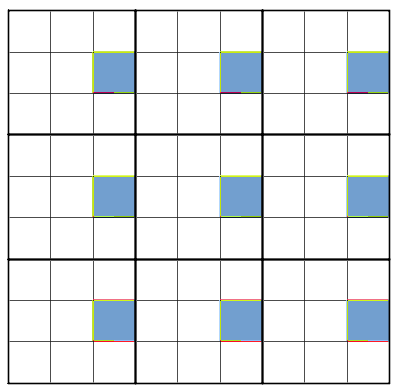
\includegraphics[width=1.4in]{sudoku.png}
\end{center}




\vspace{6pt}
{\bf Question 2: Long set operations.} Denote $A_1 = \{ 1 \}$, $A_2 = \{ 1,2 \}$, etc. 
In general, $A_k = \{ 1,2,\ldots,k\}$.\\ 
By $A \oplus B = (A - B) \cup (B-A)$
we denote the symmetric difference: All elements that belong to just one of the
sets $A,B$ (but not the other one). 
Consider this set:
$$S = \bigoplus\limits_{j=1}^{100} A_j = A_1 \oplus A_2 \oplus \ldots \oplus A_{100}.$$
Write a comma-separated list of the $10$ smallest elements of $S$ in 
increasing order.

\vspace{6pt}
{\bf Question 3: Using recurrent formula.}
Find the first $5$ members of this sequence: 
$$\left\{ \begin{array}{l} 
f(0) = 1,\\
f(1) = 4,\\
f(n) = f(n - 1) \cdot f(n - 2) + 1,\; \forall n \geq 2.
\end{array} \right.$$

Write comma-separated values $f(0),f(1),f(2),f(3),f(4)$.

\vspace{6pt}
{\bf Question 4: Reccurent sequence.} A sequence of real numbers 
$f\,:\,\mathbb{N} \rightarrow \mathbb{R}$ satisfies 
the following properties:\\
{\bf (A)} $f(k+2) = f(k) + f(k+1)$ for all integers $k \geq 2$.\\
{\bf (B)} $f(n)$ is a growing geometric progression: Namely $f(1) = f(0) \cdot q$, 
$f(2) = f(0) \cdot q^2$ and so on.


Find the quotient of this geometric progression. Round it to 
the nearest thousandth (i.e. specify the first three digits after the decimal point). 

\vspace{6pt}
{\bf Question 5: Finding a limit.} Define the following sequence: 
$$\left\{ \begin{array}{l} 
x_0 = 1,\\
x_{n+1} = \frac{1}{2} \left( x_n + \frac{2}{x_n}\right),\;\text{if}\;n\geq 0\\
\end{array} \right.$$
Assume that there exists limit $L = \lim_{n \rightarrow \infty} x_n$.\\
Find that limit $L$ and round it to 
the nearest thousandth. 

\vspace{6pt}
{\bf Question 6: Find recurrent formulas.} 
We define three sequences $(a_n)_{n \in \mathbb{N}}$, 
$(b_n)_{n \in \mathbb{N}}$, $(c_n)_{n \in \mathbb{N}}$ explicitly. 
Find their recurrent formulas that allow to find next members of the 
sequence in terms of the previous ones.
\begin{itemize}
\item ${\displaystyle a_n = 2^{\frac{1}{2^n}}}$, where $n \geq 0$. 
\item $b_0 = 1$, $b_1 = 111$, $b_2 = 11111$, $b_3 = 1111111$, etc. 
(In general, the $k$th member $b_k$ has $2k+1$ digits ``1'' in its decimal notation). 
\item $c_n = n^2 + n$. 
\end{itemize}

\begin{tabular}{|l|l|} \hline
{\bf Initial member} & {\bf Recurrent expression} \\ \hline
$a_0 = \ldots$ & $a_{n+1} = \ldots$ (express via $a_n$ etc.) \\ \hline
$b_0 = \ldots$ & $b_{n+1} = \ldots$ \\ \hline 
$c_0 = \ldots$ & $c_{n+1} = \ldots$ \\ \hline 
\end{tabular}

\vspace{6pt}
{\bf Question 7: Taylor series} There is a formula known from calculus (practically 
used to compute $y = \sin x$) for each $x \in \mathbb{R}$. 
$$\sin x = \sum\limits_{n=0}^{\infty} \frac{(-1)^n \cdot x^{2n+1}}{(2n+1)!} = x - \frac{x^3}{3!}
+ \frac{x^5}{5!} - \ldots$$

Use Python or Scala to add the first $20$ terms of this infinite sum
to compute $\sin 30^{\circ}$. Round the answer
to the nearest thousandth.
(Taylor series expects to have argument $x$ in radians, so you have to convert degrees to radians 
before using the formula.)






\end{document}

